\documentclass{report}

% Packages
\usepackage{import}
\usepackage{xcolor}
\usepackage{cancel}
\usepackage{mathtools}
\usepackage{hyperref}
\usepackage{setspace}
\usepackage{float}
\usepackage{parskip}
\setlength{\parindent}{0pt}
\usepackage{scalerel}

\renewcommand{\vec}{\mathbf}
\DeclareMathOperator{\vectorprojection}{proj}
\NewDocumentCommand{\proj}{s e{_} m}{%
    \IfBooleanTF{#1}{#3_{\stretchrel*{\parallel}{\perp}#2}}{\vectorprojection_{#2}#3}
}
\renewcommand{\Re}{\operatorname{Re}}
\renewcommand{\Im}{\operatorname{Im}}
\renewcommand{\Arg}{\operatorname{Arg}}

% Custom perms and combs commands
\newcommand\Myperm[2][^n]{\prescript{#1\mkern-2.5mu}{}P_{#2}}
\newcommand\Mycomb[2]{\prescript{#1\mkern-0.5mu}{}C_{#2}}
% Custom column vector command
\newcommand{\cvec}[1]{ \begin{pmatrix} #1 \end{pmatrix} }
% Custom determinant command
\newcommand{\det}[1]{ \begin{vmatrix} #1 \end{vmatrix} }

% Colors
\definecolor{yorhabg}{HTML}{131314}
\definecolor{yorhafg}{HTML}{C9C7CD}
\definecolor{yorhagrid}{HTML}{B5AF9C}
\definecolor{mred}{HTML}{D67069}
\definecolor{mblue}{HTML}{6887A1}

\usepackage[dvipsnames]{xcolor}
\definecolor{pastel_red}{RGB}{255, 173, 173}
\definecolor{pastel_orange}{RGB}{255, 214, 165}
\definecolor{pastel_yellow}{RGB}{253, 255, 182}
\definecolor{pastel_green}{RGB}{176, 217, 176}
\definecolor{pastel_blue}{RGB}{167, 199, 231}
\definecolor{pastel_purple}{RGB}{222, 218, 244}

\pagecolor{yorhabg}		% Set background color
\color{yorhafg}

\import{preamble.sty}

\usepackage[T1]{fontenc}			% Font package

\usepackage{fouriernc}

\usepackage{sectsty}
\usepackage{graphicx}
\usepackage{amsmath}
\usepackage{amsfonts}
\usepackage{amssymb}
\usepackage[skins, most]{tcolorbox}

\DeclareMathOperator{\sgn}{sgn}

\usepackage{tikz}
\usepackage{eso-pic}
\usetikzlibrary{calc, shadows.blur}
\usetikzlibrary{angles, quotes}
\usetikzlibrary{3d}

% Margins
\topmargin=0in
\evensidemargin=0in
\oddsidemargin=0in
\textwidth=6.5in
\textheight=9.0in
\headsep=0.25in

\AtBeginEnvironment{tcolorbox}{\small}

\newtcolorbox{imp}{enhanced,arc=0mm,colback=yorhabg,colframe=mred,leftrule=10mm,coltext=yorhafg,%
overlay={\node[anchor=west,outer sep=2pt] at (frame.west) {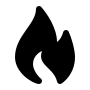
\includegraphics[width=6mm]{images/imageb.png}}; }}

\newtcolorbox{shortcut}{enhanced,arc=0mm,colback=yorhabg,colframe=mred,leftrule=10mm,coltext=yorhafg, coltitle=yorhabg, title=\texttt{Shortcut.}, 
overlay={\node[anchor=west,outer sep=2pt] at (frame.west) {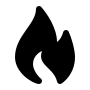
\includegraphics[width=6mm]{images/imageb.png}}; }}

\newtcolorbox{question}[1]{
    enhanced, 
    colback=yorhabg,
    colframe=mblue,
    coltext=yorhafg,
    coltitle=yorhabg,
    attach boxed title to top left={yshift*=-\tcboxedtitleheight}, 
    title=\texttt{#1},
    boxed title size=title,
    boxed title style={%
        rounded corners=northeast, 
        rounded corners=northwest, 
        colback=tcbcolframe, 
        boxrule=0pt,
    },
    underlay boxed title={%
        \path[fill=tcbcolframe] (title.south west)--(title.south east) 
            to[out=0, in=180] ([xshift=5mm]title.east)--
            (title.center-|frame.east)
            [rounded corners=5pt] |- 
            (frame.north) -| cycle; 
    },
}

\newcommand\bb[1]{\textcolor{yorhafg}{\textbf{#1}}}

\title{\textbf{MATH1141: Higher Mathematics 1A - Algebra}}
\author{L. Cheung}
\date{\today}

\begin{document}

\maketitle
\tableofcontents
\newpage

\chapter{Introduction to Vectors}

\section{Vector quantities}

	\begin{itemize}
		\item A \textbf{scalar} quantity is anything that can be specified by a single number
		\item A \textbf{vector} quantity is specified by both a magnitude and direction
	\end{itemize}

	\subsection{Geometric vectors}
	
		\begin{itemize}
			\item A geometric vector is often represented by an arrow or a directed line segment
			\item The length of the arrow represents the magnitude of the vector and the arrow points in the direction of the vector
			\item In these notes, vectors will be denoted as $\textbf{v}$
			\item Two vectors are equal if they share the same direction and magnitude. Hence, a translation of a vector would be the same vector.
		\end{itemize}

		Vectors $\textbf{u}$ and $\textbf{v}$ can be added "head to tail" to produce a new vector $\textbf{u} + \textbf{v}$

		\begin{figure}[H]
			\begin{center}
				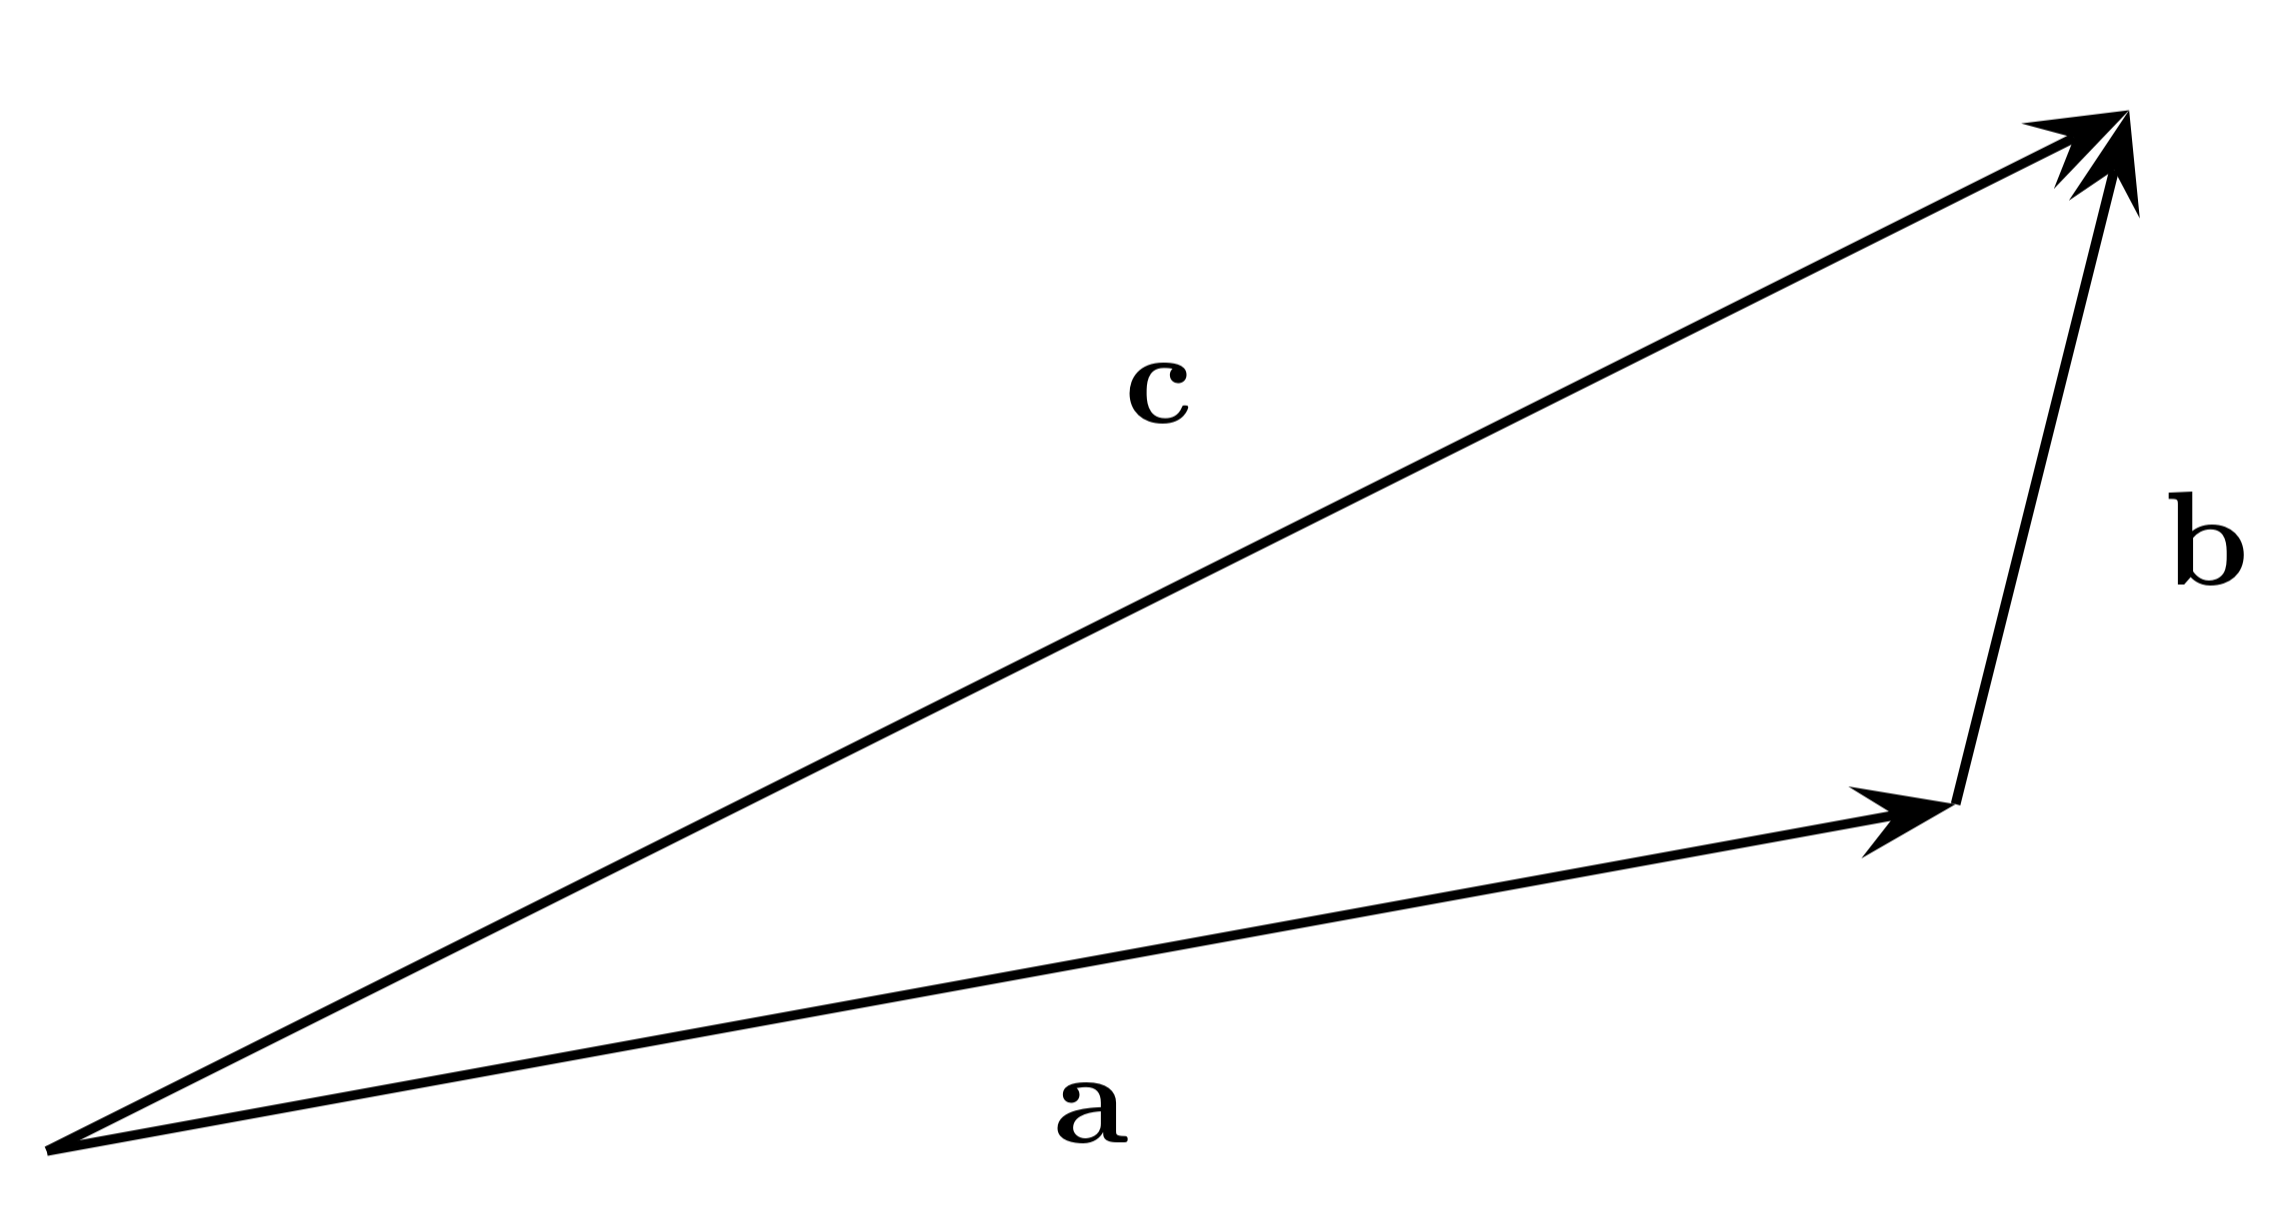
\includegraphics[width=0.8\textwidth]{images/vector_addition.png}
			\end{center}
		\end{figure}
		\\ \\
		The zero vector $\textbf{0}$ has no length and is the only vector with no specific direction. Adding the zero vector to a vector does not change it.
		\\ \\
		Scalar multiplication is the process of multiplying a vector $\textbf{v}$ by a scale $\lambda \in \mathbb{R}$. If $\lambda \geq 0$, then $\lambda \textbf{v}$ denotes the vector with the same direction, but magnitude is scaled by $\lambda$, ie. $|\lambda \textbf{v}| = \lambda |\textbf{v}|$.

		\subsubsection{Properties of vector arithmetic}

			Vector manipulation is defined similarly to regular numbers (the names of these laws should be memorised):
			
				\begin{itemize}
					\item \textbf{Commutative law}: $\textbf{v} + \textbf{w} = \textbf{w} = \textbf{v}$
					\item \textbf{Additive Associative law}: $(\textbf{u} + \textbf{v}) + \textbf{w} = \textbf{u} + (\textbf{v} = \textbf{w})$
					\item \textbf{Multiplicative Associative law}: $\lambda (\mu \textbf{v}) = (\lambda \mu) \textbf{v} \coloneq \lambda \mu \textbf{v}$
					\item \textbf{Distributive law}:
						\begin{itemize}
							\item Vector $\rightarrow$ $\lambda (\textbf{v} + \textbf{w}) = \lambda \textbf{v} + \lambda \textbf{w}$
							\item Scalar $\rightarrow$ $(\lambda + \mu) \textbf{v} = \lambda \textbf{v} + \mu \textbf{v}$
						\end{itemize}
				\end{itemize}

			Two vectors $\textbf{a}$, $\textbf{b}$ are parallel if there exists a scalar $\lambda$ such that either $\textbf{a} = \lambda \textbf{b}$ or $\textbf{b} = \lambda \textbf{a}$.

		\subsubsection{Coordinates}
			
			The place coordinates on a plane the following must be specified:
				\begin{itemize}
					\item an origin point $O$
					\item a pair of vectors $\textbf{i}$ and $\textbf{j}$ that both have a unit length and are at right angles to each other (it is conventional to choose $\textbf{j}$ at $\frac{\pi}{2}$) anticlockwise from $\textbf{i}$
				\end{itemize}
			\\ \\
			Every geometric vector $\textbf{a}$ in the plane can be written as $\textbf{a} = a_1 \textbf{i} + a_2 \textbf{j} = \begin{pmatrix}a_1\\a_2\end{pmatrix}$.

\section{Vector quantities and $\mathbb{R}^n$}
		
	Coordinate vectors can be generalised to be any number of components. Let $n$ be a positive integer. An n-tuple or n-vector is an ordered list of $n$ numbers $a_1, a_2, \dots ,a_n$ and can be either written as a row or column vector
	\\ \\
	The set of all n-tuples is denoted $\mathbb{R}^n$. Thus

		\begin{align*}
			\begin{pmatrix}0\\0\end{pmatrix} \in \mathbb{R}^2, \qquad \begin{pmatrix}1\\2\\3\end{pmatrix} \in \mathbb{R}^3, \qquad \begin{pmatrix}0\\1\\-1\\\pi\end{pmatrix} \in \mathbb{R}^4
		\end{align*}

	\subsection{Arithmetic on \mathbb{R}^n}

		Vector addition and scalar multiplication in $\mathbb{R}^n$ is defined coordinatewise, as previously demonstrated in $\mathbb{R}^2$ and $\mathbb{R}^3$.

		\begin{align*}
			\begin{pmatrix}a_1\\a_2\\\dots\\a_n\end{pmatrix} + \begin{pmatrix}b_1\\b_2\\\dots\\b_n\end{pmatrix} \coloneq \cvec{a_1+b_1\\a_2+b_2\\\dots\\a_n+b_n}
		\end{align*}
		\\ \\
		The 'zero element' is $\mathbf{0} = \cvec{0\\\dots\\0}$, and the negative is given by $-\cvec{a_1\\\dots\\a_n} = \cvec{-a_1\\\dots\\-a_n}$
		\\ \\
		Note that each $\mathbb{R}^n$ is a separate system, eg. a 3-tuple cannot be added to a 7-tuple
		\\ \\
		The length of a vector $\mathbf{a}$ is defined as $|\mathbf{a}| = \sqrt{a_1^2 + a_2^2 + \dots + a_n^2}$

	\subsection{Lines in $\mathbb{R}^n$}

		A line $L$ in $\mathbb{R}^n$ is determined by:
			\begin{itemize}
				\item a point $A$ on the line, eg. with $\mathbf{a}$ = \overrightarrow{OA}
				\item a direction, given by a non-zero vector $v$
			\end{itemize}

		\begin{align*}
			\mathbf{x} = \mathbf{a} + \lambda \mathbf{v}, \quad \lambda \in \mathbb{R}
		\end{align*}
		\\ \\
		This form is referred to as \mathbf{parametric vector form} of the line $L$.
		\\ \\
		A line in $\mathbb{R}^n$ is any set of the form
		\begin{align*}
			\left\{ \mathbf{x} \in \mathbb{R}^n | \mathbf{x} = \mathbf{a} + \lambda \mathbf{v}, \quad \lambda \in \mathbb{R} ,\; \mathbf{v} \neq \mathbf{0},\; \mathbf{a} \in \mathbb{R}^n \right\}
		\end{align*}

	\subsection{Parametric to Cartesian form}

		\begin{question}{Example}
			Write the line $\mathbf{x} = \cvec{1\\-1} + \lambda \cvec{2\\1}$, $\lambda \in \mathbb{R}$ in Cartesian form

			\begin{align*}
				\text{Let } \cvec{x\\y} &= \cvec{1\\-1} + \lambda \cvec{2\\1} = \cvec{1+2\lambda\\-1+\lambda}	\\
								\lambda &= \frac{x-1}{2} = y + 1
			\end{align*}
		\end{question}

		\begin{question}{Example}
			Consider $\mathbf{x} = \cvec{1\\-1} + \lambda \cvec{0\\1}$, $\lambda \in \mathbb{R}$
			\begin{align*}
				\cvec{x\\y} = \cvec{1\\-1+\lambda}
			\end{align*}
			In this case, $x = 1$.
		\end{question}

	\subsection{Cartesian form for lines and planes in $\mathbb{R}^3$}

		A plane in xyz-space can be described by the equation
			\begin{align*}
				ax + by + cz = d
			\end{align*}
		where not all $a$, $b$, $c$ are $0$. This is called the Cartesian form for the plane. The Cartesian form for a line in $\mathbb{R}^n$ can be defined as the intersection of two planes ($P_1 \cap P_2$). Usually, this can be written in the form
			\begin{align*}
				\frac{x-a_1}{v_1} = \frac{y-a_2}{v_2} = \frac{z-a_3}{v_3}
			\end{align*}
		for some constants $a_i$, $v_i$.

		\begin{question}{Example}
			Find the parametric form for $\frac{x-2}{3} = \frac{y+1}{6} = \frac{z-3}{-2}$
			\begin{align*}
				\lambda &= \frac{x-2}{3} = \frac{y+1}{6} = \frac{z-3}{-2}	\\
				\mathbf{x} &= \cvec{x\\y\\z} = \cvec{3\lambda+2\\6\lambda_1\\-2\lambda+3} = \cvec{2\\-1\\3} + \lambda \cvec{3\\6\\-2}, \quad \lambda \in \mathbb{R}
			\end{align*}
		\end{question}

	\subsection{Parametric to Cartesian form for lines in $\mathbb{R}^3$}

		\begin{question}{Example}
			Find a Cartesian form for $\mathbf{x} = \cvec{1\\2\\3} + \lambda \cvec{4\\5\\6}$, $\lambda \in \mathbb{R}$
			\begin{align*}
				\cvec{4\lambda+1\\5\lambda+2\\6\lambda+3} = \cvec{x\\y\\z}
			\end{align*}
			\begin{align*}
				\lambda = \frac{x-1}{4} = \frac{y-2}{5} = \frac{z-3}{6}
			\end{align*}
		\end{question}
		\begin{question}{Example}
			Consider $\mathbf{x} = \cvec{1\\2\\3} + \lambda \cvec{4\\5\\0}$
			\begin{align*}
				\lambda = \frac{x-1}{4} = \frac{y-2}{5}, \quad z=3
			\end{align*}
		\end{question}

	\subsection{Linear combination}

		Suppose that $\mathbf{v_1}, \mathbf{v_2}, \dots, \mathbf{v_k} \in \mathbb{R}^n$. A linear combination of these vectors is a vector of the form
		\begin{align*}
			\lambda_1 \mathbf{v_1} + \lambda_2 \mathbf{v_2} + \dots + \lambda_k \mathbf{v_k}, \quad \lambda_1, \dots, \lambda_k \in \mathbb{R}
		\end{align*}

	\subsection{Span}

		The span of $\mathbf{v_1}, \mathbf{v_2}, \dots, \mathbf{v_k}$ is the set of all linear combinations of $\mathbf{v_1}, \mathbf{v_2}, \dots, \mathbf{v_k}$, ie.
			\begin{align*}
				\text{span}(\mathbf{v_1}, \mathbf{v_2}, \dots, \mathbf{v_k}) = \left\{\lambda_1 \mathbf{v_1}, \lambda_2 \mathbf{v_2}, \dots, \lambda_k \mathbf{v_k} | \lambda_1, \dots, \lambda_k \in \mathbb{R} \right\}
			\end{align*}
		Note that $\text{span}(\emptyset) = \left\{ \mathbf{0} \right\}$

	\subsection{Planes in $\mathbb{R}^n$}

		A plane in $\mathbb{R}^n$ is defined to be a set of the form
			\begin{align*}
				S = \left\{ \mathbf{a} + \lambda_1 \mathbf{v_1} + \lambda_2 \mathbf{v_2} | \lambda_1, \lambda_2 \in \mathbb{R} \right\}
			\end{align*}
		where $\mathbf{a}$, $\mathbf{v_1}$ and $\mathbf{v_2}$ are fixed vectors in $\mathbb{R}^n$, and $\mathbf{v_1}$ and $\mathbf{v_2}$ are not parallel.
		\\ \\
		The expression $\mathbf{x} = \mathbf{a} + \lambda_1 \mathbf{v_1} + \lambda_2 \mathbf{v_2}$, $\lambda_1, \lambda_2 \in \mathbb{R}$ is a parametric vector form for the plane through $\mathbf{a}$ parallel to the vectors $\mathbf{v_1}$ and $\mathbf{v_2}$.

		\begin{question}{Example}
			Find a parametric vector equation for the plane containing the point $\mathbf{a} = \cvec{1\\2\\1}$, and line $\mathbf{x} = \cvec{0\\1\\2} + \lambda \cvec{3\\-4\\2}$, $\lambda \in \mathbb{R}$.
			\begin{align*}
				\text{Let direction } \mathbf{v_2} &= \cvec{1\\2\\1} - \cvec{0\\1\\2} = \cvec{1\\1\\-1}	\\
				\mathbf{x} &= \cvec{0\\1\\2} + \lambda_1 \cvec{3\\-4\\2} + \lambda_2 \cvec{1\\1\\-1}, \quad \lambda_1, \lambda_2 \in \mathbb{R}
			\end{align*}
		\end{question}

		\begin{question}{Example}
			Find the Cartesian equation of the plane in $\mathbb{R}^3$: $\cvec{x\\y\\z} = \cvec{1\\2\\3} + \lambda_1 \cvec{-1\\1\\-1} + \lambda_2 \cvec{3\\2\\1}$, $\lambda_1, \lambda_2 \in \mathbb{R}$.

			Equating coordinates and adding:
			\begin{align*}
				x + y &= 3 + 5 \lambda_2	\\
				y + z &= 5 + 3 \lambda_2
			\end{align*}

			Hence $3(x+y) - 5(y+z) = 3(3) = 5(5) = -16$
			\begin{align*}
				\therefore -16 = 3x - 2y - 5z
			\end{align*}
		\end{question}

\chapter{Vector Geometry}

\section{Angles via cosine rule}

	Let $\mathbf{a} = \overrightarrow{OA}, \mathbf{b} = \overrightarrow{OB} \in \mathbb{R}^n$ be non-zero. The cosine rule is as follows
		\begin{align*}
			|\mathbf{b} - \mathbf{a}|^2 = |\mathbf{a}|^2 + |\mathbf{b}|^2 - 2|\mathbf{a}||\mathbf{b}| \cos{\theta}
		\end{align*}

	The formula for the length of a vector gives
		\begin{align*}
			\sum_i (b_i - a_i)^2 = \sum_i a_i^2 + \sum_i b_i^2 - 2|\mathbf{a}||\mathbf{b}| \cos{\theta}
		\end{align*}

	Cancelling gives $-2 |\mathbf{a}||\mathbf{b}| \cos{\theta} = \sum_i -2 a_i b_i$ so
		\begin{align*}
			\cos{\theta} = \frac{\sum_i a_i b_i}{|\mathbf{a}||\mathbf{b}|}
		\end{align*}

	$\theta$ is solvable as long as RHS lies in $[-1,1] \quad$ (Cauchy-Schwarz theorem)

	\\ \\
	The dot product of two vectors $\mathbf{a}, \mathbf{b} \in \mathbb{R}^n$ is defined to be
		\begin{align*}
			\mathbf{a} \cdot \mathbf{b} = \sum_i a_i b_i
		\end{align*}
	
	Hence, the angle between two non-zero vectors $\mathbf{a} = \overrightarrow{OA}, \mathbf{b} = \overrightarrow{OB} \in \mathbb{R}^n$ is
		\begin{align*}
			\theta = \cos^{-1}{\left(\frac{\mathbf{a} \cdot \mathbf{b}}{|\mathbf{a}||\mathbf{b}|}\right)}
		\end{align*}

	\subsubsection{Properties of the dot product}

		Suppose $\mathbf{a}, \mathbf{b}, \mathbf{c} \in \mathbb{R}^n$. Then
			\begin{itemize}
				\item $\mathbf{a} \cdot \mathbf{b} = \mathbf{b} \cdot \mathbf{a}$
				\item $\mathbf{a} \cdot (\lambda \mathbf{b}) = (\lambda \mathbf{a}) \cdot \mathbf{b} = \lambda(\mathbf{a} \cdot \mathbf{b})$
				\item $\mathbf{a} \cdot (\mathbf{b} + \mathbf{c}) = \mathbf{a} \cdot \mathbf{b} + \mathbf{a} \cdot \mathbf{c}$
				\item $\mathbf{a} \cdot \mathbf{a} = |\mathbf{a}|^2 \geq 0$
			\end{itemize}

	\subsection{Cauchy-Schwarz theorem}

		The Cauchy-Schwarz theorem is as follows
			\begin{align*}
				-|\mathbf{a}||\mathbf{b}| \leq \mathbf{a} \cdot \mathbf{b} \leq |\mathbf{a}||\mathbf{b}|
			\end{align*}
		\\ \\
		\begin{question}{Proof}
			The inequality holds when $\mathbf{b} = \mathbf{0}$ so it is assumed $\mathbf{b} \neq \mathbf{0}$. Consider the real function of (the real variable) $\lambda$
			\begin{align*}
				q(\lambda) &= |\mathbf{a} = \lambda \mathbf{b}|^2 \geq 0	\\
				q(\lambda) &= (\mathbf{a} - \lambda \mathbf{b}) \cdot (\mathbf{a} - \lambda \mathbf{b})	\\
						   &= |\mathbf{a}|^2 - 2 \lambda \mathbf{a} \cdot \mathbf{b} + \lambda^2 |\mathbf{b}|^2
			\end{align*}
			The discriminant of this quadratic function of $\lambda$ must be non-positive, hence
			\begin{align*}
				0 \geq (-2\mathbf{a} \cdot \mathbf{b})^2 - 4|\mathbf{a}|^2|\mathbf{b}|^2 = 4(\mathbf{a} \cdot \mathbf{b})^2 - 4|\mathbf{a}|^2|\mathbf{b}|^2 \Longrightarrow (\mathbf{a} \cdot \mathbf{b})^2 \leq |\mathbf{a}|^2|\mathbf{b}|^2
			\end{align*}
		\end{question}

\section{Orthogonality}

	Two vectors $\mathbf{a}, \mathbf{b} \in \mathbb{R}^n$ are said to be orthogonal if $\mathbf{a} \cdot \mathbf{b} = 0$, ie. the angle between them is $\frac{\pi}{2}$

	\begin{question}{Example}
		Consider $\mathbf{a} = \cvec{1\\1\\-1\\1}$ and $\mathbf{b} = \cvec{-2\\1\\1\\2}$
		\begin{align*}
			\mathbf{a} \cdot \mathbf{b} = (1 \times -2) + (1 \times 1) + (-1 \times 1) + (1 \times 2) = 0
		\end{align*}
		therefore, $\mathbf{a}$ and $\mathbf{b}$ are orthogonal.
	\end{question}

	If $\mathbf{a}, \mathbf{b} \in \mathbb{R}^n$ are orthogonal then
	\begin{align*}
		|\mathbf{a} + \mathbf{b}|^2 = |\mathbf{a}|^2 + |\mathbf{b}|^2
	\end{align*}

	\subsection{Orthonormal sets of vectors}

		The vectors $\mathbf{v_1}, \dots, \mathbf{v_k} \in \mathbb{R}^n$ form an orthogonal set if they are mutually orthogonal. Furthermore, if they all have length 1, the vectors are orthonormal.

		Equivalently, $\mathbf{v_1}, \dots, \mathbf{v_k}$ are orthonormal if
		\begin{align*}
			v_i \cdot v_j = \delta_{ij} \coloneq \begin{cases}1,\quad & \text{ if } i = j	\\ 0, & \text{ if } i \neq j\end{cases}
		\end{align*}
		[$\delta_{ij}$ is called the Kronecker delta symbol]


		\subsubsection{Arithmetic prperties of the cross product}
			
			For $\vec{a}, \vec{b}, \vec{c} \in \mathbb{R}$ and $\lambda \in \mathbb{R}$

				\begin{itemize}
					\item $\vec{a} \times \vec{a} = 0$
					\item $\times$ is distributive:
						\begin{itemize}
							\item $\vec{a} \times (\vec{b} + \vec{c}) = (\vec{a} \times \vec{b}) + (\vec{a} \times \vec{c})$
							\item $(\vec{a} + \vec{b}) \times \vec{c} = (\vec{a} \times \vec{c}) + (\vec{b} \times \vec{c})$
						\end{itemize}
					\item $(\lambda \vec{a}) \times \vec{b} = \lambda (\vec{a} \times \vec{v}) = \vec{a} \times (\lambda \vec{b})$
					\item Since $\vec{a} \times \vec{b} = -\vec{b} \times \vec{a}$, $\times$ is not commutative
					\item The cross product is not associative
				\end{itemize}

		\subsubsection{The magnitude of $\vec{a} \times \vec{b}$}

			Suppose that $\vec{a}, \vec{b} \in \mathbb{R}^3$ are nonzero, with angle $\theta$ between them. Then $|\vec{a} \times \vec{b}| = |\vec{a}||\vec{b}| \sin \theta$. Since $\theta \in [0, \pi]$ in $\mathbb{R}^3$, therefore $\sin \theta \geq 0$. Thus, it is sufficient that
			
				\begin{align*}
					|\vec{a} \times \vec{b}|^2 = |\vec{a}|^2 |\vec{b}|^2 \sin^2 \theta
				\end{align*}

		\subsubsection{Areas of parallelgroms via cross product}

			The area of a parallelogram is

				\begin{align*}
					A = \text{base} \times \text{perp height} = |\vec{a}||\vec{b}| \sin \theta
				\end{align*}

		\subsubsection{Direction of $\vec{a} \times \vec{b}$}

			Row swapping of determinants gives the following

			\begin{itemize}
				\item $\vec{a} \dot (\vec{b} \times \vec{c}) = - \vec{a} \dot (\vec{c} \times \vec{b}) = \vec{c} \dot (\vec{a} \times \vec{b})$
				\item $\vec{a} \dot (\vec{a} \times \vec{b}) = 0 = \vec{a} \dot (\vec{b} \times \vec{b})$
			\end{itemize}

			The vector $\vec{a} \times \vec{b}$ is orthogonal to both $\vec{a}$ and $\vec{b}$

		\subsubsection{Parametric to Cartesian form via point-normal}

			\begin{question}{Example}
				Find a point-normal, and hence a Cartesian form for the plane $\vec{x} = \cvec{-3\\1\\2} + \lambda_1 \cvec{1\\1\\-2} + \lambda_2 \cvec{4\\0\\3}, \quad \lambda_1, \lambda_2 \in \mathbb{R}$

				A point on the line is $\vec{a} = \cvec{-3\\1\\2}$
				\begin{flalign*}
					\text{A vector normal to the plane is }\vec{n} &= \cvec{1\\1\\-2} \times \cvec{4\\0\\3}		& \\
				\end{flalign*}

			\end{question}

\chapter{Complex Numbers}
	
	\subsection{Fields}
		
		A field is a non empty set for which a rule for addition and multiplication are defined. The field must define values for the following axioms

		\begin{enumerate}
			\item \textbf{Closure under Addition.} If $x, y \in \mathbb{F}$ then $x + y \in \mathbb{F}$.
			\item \textbf{Associative Law of Addition.} $(x + y) + z = x + (y + z)$ for all $x, y, z \in \mathbb{F}$.
			\item \textbf{Commutative Law of Addition.} $x + y = y + x$ for all $x, y \in \mathbb{F}$.
			\item \textbf{Existence of a Zero.} There exists an element of $\mathbb{F}$ (usually written as $0$) such that $0 + x = x + 0 = x$ for all $x \in \mathbb{F}$.
			\item \textbf{Existence of a Negative.} For each $x \in \mathbb{F}$, there exists an element $w \in \mathbb{F}$ (usually written as $-x$) such that x + w = w + x = 0.
			\item \textbf{Closure under Multiplication.} If $x, y \in \mathbb{F}$ then $xy \in \mathbb{F}$.
			\item \textbf{Associative Law of Multiplication.} $x(yz) = (xy)z$ for all $x, y, z \in \mathbb{F}$.
			\item \textbf{Commutative Law of Multiplication.} $xy = yx$ for all $x, y \in \mathbb{F}$.
			\item \textbf{Existence of a One.} There exists a non-zero element of $\mathbb{F}$ (usually written as $1$) such that $x1 = 1x = x$ for all $x \in \mathbb{F}$.
			\item \textbf{Existence of an Inverse for Multiplication.} For each non-zero $x \in \mathbb{F}$, there exists an element $w$ of $\mathbb{F}$ (usually written as $1/x$ or $x^{-1}$) such that $xw = wx = 1$.
			\item \textbf{Distributive Law.} $x(y + z) = xy + xz$ for all $x, y, z \in \mathbb{F}$.
			\item \textbf{Distributive Law.} $(x + y)z = xz + yz$ for all $x, y, z \in \mathbb{F}$.
		\end{enumerate}

	\subsection{Complex numbers}
		
	A complex number is a formal expression of the form $a + bi$ for some $a,b \in \mathbb{R}$. In particular, two such numbers $a+bi$, $a'+b' i$ are equal iff $a = a', b = b'$ as real numbers. The real part of $a+bi$ is $\text{Re}(a+bi) = a$ and the imaginary part is $\text{Im}(a+bi) = b$.

		\subsubsection{Arithmetic of complex numbers}
			
			Given the complex numbers $a+bi, a'+b'i$, addition and multiplication is defined as follows

				\begin{align*}
					(a+bi)+(a'+b'i) &= (a+a') + (b+b')i	\\
					(a+bi)(a'+b'i) &= (aa'-bb') + (ab' + a'b)i
				\end{align*}

	The complex set $\mathbb{C}$ extends the real number system since complex numbers of form $a + 0i$ add and multiply the same way as real numbers. It contains the number $i$ satisfying $i^2 = -1$

		\subsubsection{Cartesian form}

			A complex number $z$ written in the form $a+bi$ with $a,b \in \mathbb{R}$ is called the Cartesian form

			\begin{question}{Example}
				Express $\frac{1+i}{1-i} - \frac{1-i}{1+i}$ in Cartesian form

				\begin{align*}
					\frac{1+i}{1-i} - \frac{1-i}{1+i} &= \frac{(1+i)^2 - (1-i)^2}{(1-i)(1+i)}	\\
													  &= \frac{(1+2i+i^2) - (1-2i+i^2)}{1^2 + 1^2}		\\
													  &= \frac{4i}{2}	\\
													  &= 2i
				\end{align*}
			\end{question}

		\subsubsection{Conjugation}

			The conjugate of a complex number $z=a+bi$ is defined as $\overline{z} = a-bi$

			\begin{itemize}
				\item $z$ is real iff $\overline{z} = z$
				\item $\overline{\overline{z}} = z$
				\item $\overline{z+w} = \overline{z} + \overline{w}$ and $\overline{z-w} = \overline{z} - \overline{w}$
				\item $\overline{zw} = \overline{z} \; \overline{w}$ and $\overline{\frac{z}{w}} = \frac{\overline{x}}{\overline{w}}$
				\item $\text{Re}(z) = \frac{1}{2}\left(z + \overline{z}\right)$ and $\text{Im}(z) = \frac{1}{2i} \left(z - \overline{z}\right)$
			\end{itemize}

			\begin{question}{Example}
				Show that for any $z \in \mathbb{C}$, $(i+5)z - (i-5)\overline{z}$ is real.
				\begin{flalign*}
					\text{Let } w &= (i+5)z - (i-5)\overline{z}	\\
					\overline{w} &= \overline{(i+5)z - (i-5)\overline{z}}	\\
								 &= (5-i)\overline{z} - (-i-5)z		\\
								 &= (i-5) \overline{z} + (i+5)z		\\
								 &= w
				\end{flalign*}
			\end{question}

	\section{The Argand diagram}

		Similarly to how real numbers can be represented on a plane, complex numbers can be represented on the complex plane (the Argand diagram).
		\\ \\
		$z = a+bi$ is represented by the point with coords $(a,b) = \left(\Re(z), \Im(z)\right)$
		\\ \\
		Adding complex numbers by adding real and imaginary parts (ie. coordinatewise) can be represented geometrically by the addition of vectors.

		\subsection{Polar form}
		
			Given the Cartesian form of a complex number $z = x + iy, \; x, y \in \mathbb{R}$, polar coordinates for $z = (r, \theta)$ can be found
				\begin{align*}
					z = r \cos \theta + \left(r \sin \theta \right) i
				\end{align*}

			Let $z = x + iy, \; x, y \in \mathbb{R}$
			\begin{itemize}
				\item The \textbf{modulus} of $z$ is defined as $|z| = r = \sqrt{x^2 + y^2}$ so $z \overline{z} = |z|^2$
				\item If $z \neq 0$, an \textbf{argument} for $z$ is any $\theta = \arg z$ so that $\tan \theta = \frac{y}{x}$
				\item Furthermore, $\theta =: \operatorname{Arg} z$ is the \textbf{principal argument} if $\theta \in (-\pi, \pi]$
			\end{itemize}

			\begin{question}{Example}
				Find the modulus and principal argument of $-1 -\sqrt{3}i$.
					\begin{flalign*}
						|-1-\sqrt{3}i| = \sqrt{1^2 + (\sqrt{3})^2} = 2	\\
						\arctan \frac{-\sqrt{3}}{-1} = \arctan \sqrt{3} = \frac{\pi}{3}		\\
						\operatorname{Arg} (-1-\sqrt{3}) = \frac{\pi}{3} - \pi = -\frac{2\pi}{3}
					\end{flalign*}
			\end{question}

		\subsection{Euler's formula}

			For $\theta \in \mathbb{R}$, it is defined $e^{i\theta} = \cos \theta + i \sin \theta$. This formula is reasonable by
			
			\begin{itemize}
				\item $e^{i \theta_1}e^{i \theta_2} = e^{i(\theta_1+\theta_2)}$
				\item (De Moivre's theorem) For $n \in \mathbb{Z},\; \left(e^{i\theta}\right)^n = e^{in\theta}$
				\item $\frac{d}{d\theta} (e^{i \theta}) = ie^{i\theta}$
			\end{itemize}

			\subsubsection{Arithmetic of polar forms}
				
				The polar form of $z$ is $z = re^{i\theta}$ where $r = |z|$ and $\theta$ is an argument of $z$. The above formulae give
				\begin{align*}
					r_1 e^{i\theta_1} r_2 e^{i\theta_2} = (r_1 r_2) e^{i(\theta_1+\theta_2)} \quad , \quad \left(re^{i\theta}\right)^{-1} = r^{-1}e^{-i\theta}
				\end{align*}
				ie. multiplication of complex numbers can be achieved by multiplying the moduli and adding the arguments. Inverting a complex number inverts the modulus and negates the argument.

				\begin{question}{Example}
					Find the exact value of $\operatorname{Arg} \frac{1+i}{1+\sqrt{3}i}$
					\begin{align*}
						\arg \frac{1+i}{1+\sqrt{3}i} &= \arg(1+i) - \arg(1+\sqrt{3}i)	\\
													 &= \frac{\pi}{4} - \frac{\pi}{3}	\\
						\Arg \frac{1+i}{1+\sqrt{3}i} &= -\frac{\pi}{12}					\\
					\end{align*}
				\end{question}

				\begin{question}{Example}
					Let $z \in \mathbb{C}$ have $|z| = 1$. Show that $w = \frac{i-z}{i+z}$ is purely imaginary in the sense that $\Re(w) = 0$ Interpret the result geometrically.

					\begin{align*}
						\Re(w) = \frac{1}{2} (w + \overline{w})		\\
						\overline{w} &= \frac{\overline{i-z}}{\overline{i+z}}	\\
									 &= \frac{-i-\overline{z}}{-i+\overline{z}} \times \frac{iz}{iz}	\\
									 &= \frac{z-i|z|^2}{z+i}		\\
									 &= -w
					\end{align*}
					Therefore, $w$ is purely imaginary
				\end{question}
				\begin{question}{Example}
					Find the complex sqaure roots $\pm z$ of $16-30i$

					\begin{align*}
						\text{Let } z = a+bi,\; a,b \in \mathbb{R} \text{ such that } z^2 = 16-30i	\\
						&\therefore 16-30i = (a+bi)^2 = a^2 + 2abi - b^2	\\
						&= a^2 - b^2 + 2abi	\\
						&\text{Real part gives: }16 = a^2 - b^2	\\
						&\text{Imaginary part gives: } -30 = 2ab \Leftrightarrow -15=ab	\\
						z = \pm (5-3i)
					\end{align*}
				\end{question}
				\begin{question}{Example}
					Solve $z^2 + (1-i)z + (-4+8i) = 0$
					\begin{align*}
						z &= \frac{-(1-i) \pm \sqrt{(1-i)^2 - 4(1)(-4+8i)}}{2(1)}	\\
						\Delta &= b^2 - 4ac = (1-i)^2 - 4(1)(-4+8i) = 1^2 + 2i + i^2 + 16 - 32i = 16-30i	\\
							   &\text{From above, } \sqrt{\Delta} = \pm (5-3i)		\\
						z &= \frac{-(1+i) \pm (5-3i)}{2} = \frac{4 - 4i}{2} \text{ or } \frac{-6+2i}{2}		\\
						  &= 2-2i, \; -3+i
					\end{align*}
				\end{question}

		\subsection{Powers of complex numbers}

			\begin{question}{Example}
				Find $w = (1+i)^{18}$
				\begin{align*}
					\text{Let } z &= 1+i = \sqrt{2}e^{i \frac{\pi}{4}}	\\
					w &= z^{18}		\\
					  &= (\sqrt{2}e^{i \frac{\pi}{4}})^{18}	\\
					  &= 2^9 e^{i \frac{9\pi}{2}}	\\
					  &= 2^9 e^{i\frac{\pi}{2}}	\\
					  &= 2^9 i
				\end{align*}
			\end{question}

		\subsection{Roots of complex numbers}
			
			\begin{question}{Example}
				Solve $z^4 = i$.
				\\ \\
				Solve in polar form for $z = re^{i\theta}, \; \pi < \theta \leq \pi$

				\qquad Equate moduli:  $1 = |i| = |z^4| = |z|^4, \; \therefore r = 1$

				\qquad Equate arguments:  $\arg(z^4) &= \arg i$	\\

				4 \Arg(z) = \frac{\pi}{2}

				\dots (got lazy, answer trivial)
			\end{question}

		\subsection{Expressing trigonometric polynomials as polynomials in $\cos \theta, \; \sin \theta$}

			A trigonometric polynomial is a linear combination of functions of the form $\cos n \theta, \; \sin n \theta$.

			\begin{question}{Example}
				Use De Moivre's theorem to show $\cos(3\theta) = 4 \cos^3\theta - 3 \cos \theta$
				\begin{align*}
					cos 3\theta &= \Re(e^{i3\theta})	\\
								&= \Re(\cos \theta + i \sin \theta)^3	\\
								&= Re(\cos^3 \theta + 3i \cos^2 \theta \sin \theta - 3 \cos \theta \sin^2 \theta - i \sin^3 theta)	\\
								&= \cos^3 \theta  - 3 \cos \theta \sin^2 \theta	\\
								&= \cos^3 \theta - 3 \cos \theta (1 - \cos^2 \theta)	\\
								&= 4 \cos^3 \theta - 3 \cos \theta
				\end{align*}
			\end{question}
\end{document}
